\documentclass{article}\usepackage[]{graphicx}\usepackage[]{color}
%% maxwidth is the original width if it is less than linewidth
%% otherwise use linewidth (to make sure the graphics do not exceed the margin)
\makeatletter
\def\maxwidth{ %
  \ifdim\Gin@nat@width>\linewidth
    \linewidth
  \else
    \Gin@nat@width
  \fi
}
\makeatother

\definecolor{fgcolor}{rgb}{0.345, 0.345, 0.345}
\newcommand{\hlnum}[1]{\textcolor[rgb]{0.686,0.059,0.569}{#1}}%
\newcommand{\hlstr}[1]{\textcolor[rgb]{0.192,0.494,0.8}{#1}}%
\newcommand{\hlcom}[1]{\textcolor[rgb]{0.678,0.584,0.686}{\textit{#1}}}%
\newcommand{\hlopt}[1]{\textcolor[rgb]{0,0,0}{#1}}%
\newcommand{\hlstd}[1]{\textcolor[rgb]{0.345,0.345,0.345}{#1}}%
\newcommand{\hlkwa}[1]{\textcolor[rgb]{0.161,0.373,0.58}{\textbf{#1}}}%
\newcommand{\hlkwb}[1]{\textcolor[rgb]{0.69,0.353,0.396}{#1}}%
\newcommand{\hlkwc}[1]{\textcolor[rgb]{0.333,0.667,0.333}{#1}}%
\newcommand{\hlkwd}[1]{\textcolor[rgb]{0.737,0.353,0.396}{\textbf{#1}}}%

\usepackage{framed}
\makeatletter
\newenvironment{kframe}{%
 \def\at@end@of@kframe{}%
 \ifinner\ifhmode%
  \def\at@end@of@kframe{\end{minipage}}%
  \begin{minipage}{\columnwidth}%
 \fi\fi%
 \def\FrameCommand##1{\hskip\@totalleftmargin \hskip-\fboxsep
 \colorbox{shadecolor}{##1}\hskip-\fboxsep
     % There is no \\@totalrightmargin, so:
     \hskip-\linewidth \hskip-\@totalleftmargin \hskip\columnwidth}%
 \MakeFramed {\advance\hsize-\width
   \@totalleftmargin\z@ \linewidth\hsize
   \@setminipage}}%
 {\par\unskip\endMakeFramed%
 \at@end@of@kframe}
\makeatother

\definecolor{shadecolor}{rgb}{.97, .97, .97}
\definecolor{messagecolor}{rgb}{0, 0, 0}
\definecolor{warningcolor}{rgb}{1, 0, 1}
\definecolor{errorcolor}{rgb}{1, 0, 0}
\newenvironment{knitrout}{}{} % an empty environment to be redefined in TeX

\usepackage{alltt}
\usepackage[margin = 1in]{geometry}
\usepackage{float}
\usepackage{graphicx}
\IfFileExists{upquote.sty}{\usepackage{upquote}}{}
\begin{document}

\title{ASSIGNMENT 1}
\author{Brandon Lampe \\ STAT 527 \\ Advanced Data Analysis I}
\maketitle


\section{Part I.}
  \begin{enumerate}
    \item \textbf{Precip:} \\
Download monthly precipitation and sulphur concentration; data from Univ. of Stockholm.
Data type changed from integer to numeric to allow for plotting.

\begin{knitrout}
\definecolor{shadecolor}{rgb}{0.969, 0.969, 0.969}\color{fgcolor}\begin{kframe}
\begin{alltt}
\hlkwd{library}\hlstd{(ggplot2)} \hlcom{#load ggplot}
\hlstd{d1} \hlkwb{<-} \hlkwd{read.csv}\hlstd{(}\hlstr{"http://statacumen.com/teach/ADA1/ADA1_HW_01_F14-1.csv"}\hlstd{)}

\hlstd{Month} \hlkwb{<-} \hlstd{d1}\hlopt{$}\hlstd{Month}
\hlstd{Precip} \hlkwb{<-} \hlkwd{as.numeric}\hlstd{(d1}\hlopt{$}\hlstd{Precip)}   \hlcom{# change type to numeric}
\hlstd{Sulphur} \hlkwb{<-} \hlkwd{as.numeric}\hlstd{(d1}\hlopt{$}\hlstd{Sulphur)} \hlcom{# change type to numeric}
\end{alltt}
\end{kframe}
\end{knitrout}

      \begin{enumerate} % problem one a
        \item Make stem-and-leaf, histogram, and boxplot for Precip data: \\ \\
% ============ figures for (a) =========
\begin{knitrout}
\definecolor{shadecolor}{rgb}{0.969, 0.969, 0.969}\color{fgcolor}\begin{kframe}
\begin{alltt}
\hlkwd{stem}\hlstd{(Precip,} \hlkwc{scale} \hlstd{=} \hlnum{2}\hlstd{)}
\end{alltt}
\begin{verbatim}
## 
##   The decimal point is 1 digit(s) to the right of the |
## 
##   1 | 29
##   2 | 35
##   3 | 556
##   4 | 
##   5 | 25
##   6 | 39
##   7 | 
##   8 | 1
\end{verbatim}
\end{kframe}
\end{knitrout}

\begin{knitrout}
\definecolor{shadecolor}{rgb}{0.969, 0.969, 0.969}\color{fgcolor}\begin{kframe}
\begin{alltt}
\hlcom{# histogram of Precip}
\hlstd{Precip.hist} \hlkwb{<-} \hlkwd{ggplot}\hlstd{(d1,} \hlkwd{aes}\hlstd{(}\hlkwc{x} \hlstd{= Precip))}
\hlstd{Precip.hist} \hlkwb{<-} \hlstd{Precip.hist} \hlopt{+} \hlkwd{geom_histogram}\hlstd{(}\hlkwc{binwidth} \hlstd{=} \hlnum{5}\hlstd{)}
\hlstd{Precip.hist} \hlkwb{<-} \hlstd{Precip.hist} \hlopt{+} \hlkwd{labs}\hlstd{(}\hlkwc{title} \hlstd{=} \hlstr{"Monthly Precipitation [mm]"}\hlstd{)}
\end{alltt}
\end{kframe}
\end{knitrout}

\begin{figure}[H]  \begin{center}
\begin{knitrout}
\definecolor{shadecolor}{rgb}{0.969, 0.969, 0.969}\color{fgcolor}
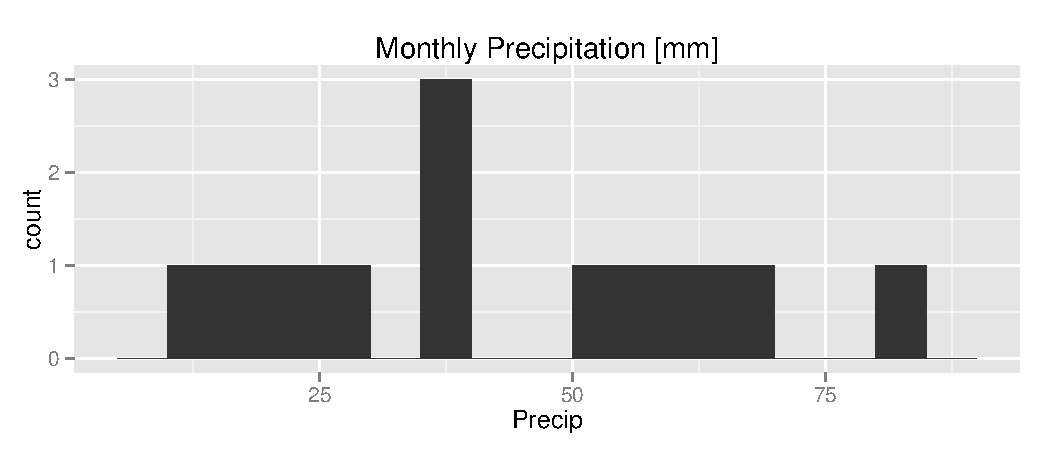
\includegraphics[width=\maxwidth]{figure/1p_hist} 

\end{knitrout}
\end{center} \vspace{-0.25in}\caption{Histogram of Precip Data} \end{figure}

\begin{knitrout}
\definecolor{shadecolor}{rgb}{0.969, 0.969, 0.969}\color{fgcolor}\begin{kframe}
\begin{alltt}
\hlstd{Precip.box} \hlkwb{<-} \hlkwd{ggplot}\hlstd{(d1,} \hlkwd{aes}\hlstd{(}\hlkwc{x} \hlstd{=} \hlstr{"in"}\hlstd{,} \hlkwc{y} \hlstd{= Precip))} \hlcom{# boxplot of Precip}
\hlstd{Precip.box} \hlkwb{<-} \hlstd{Precip.box} \hlopt{+} \hlkwd{geom_boxplot}\hlstd{()}
\hlstd{Precip.box} \hlkwb{<-} \hlstd{Precip.box} \hlopt{+} \hlkwd{coord_flip}\hlstd{()}
\hlstd{Precip.box} \hlkwb{<-} \hlstd{Precip.box} \hlopt{+} \hlkwd{labs}\hlstd{(}\hlkwc{title} \hlstd{=} \hlstr{"Monthly Precipitation [mm]"}\hlstd{)}
\end{alltt}
\end{kframe}
\end{knitrout}

\begin{figure}[H]  \begin{center}
\begin{knitrout}
\definecolor{shadecolor}{rgb}{0.969, 0.969, 0.969}\color{fgcolor}
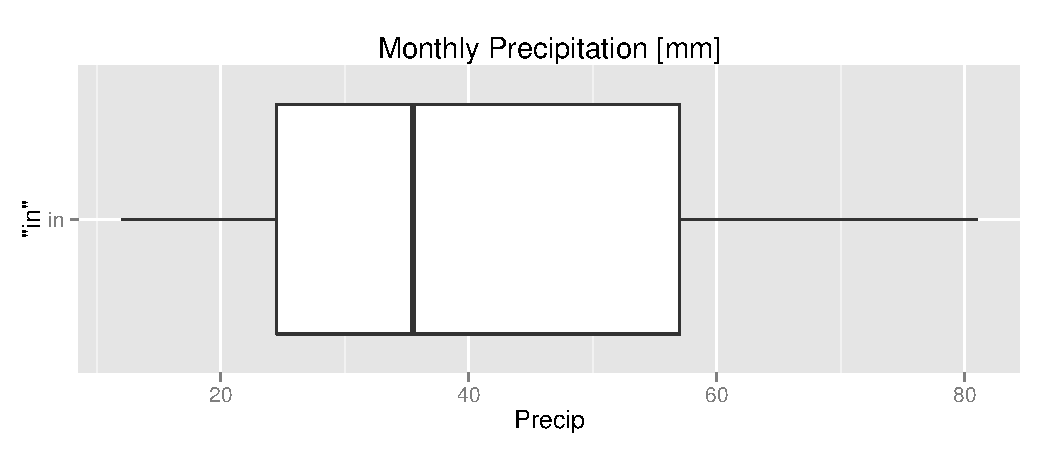
\includegraphics[width=\maxwidth]{figure/1p_box} 

\end{knitrout}
\end{center} \vspace{-0.15in} \caption{Boxplot of Precip Data} \end{figure}
% ======== end (a)

      \item Compute mean, median, standard deviation, and IQR for Precip data:
        \begin{itemize}
          \item mean: 42.08
          \item median:  35.5
          \item standard deviation:  21.69
          \item inter quartile range:  32.5
        \end{itemize}
\begin{knitrout}
\definecolor{shadecolor}{rgb}{0.969, 0.969, 0.969}\color{fgcolor}\begin{kframe}
\begin{alltt}
\hlkwd{mean}\hlstd{(Precip)}    \hlcom{# mean of precip}
\end{alltt}
\begin{verbatim}
## [1] 42.08
\end{verbatim}
\begin{alltt}
\hlkwd{median}\hlstd{(Precip)}  \hlcom{# median of precip}
\end{alltt}
\begin{verbatim}
## [1] 35.5
\end{verbatim}
\begin{alltt}
\hlkwd{sd}\hlstd{(Precip)}      \hlcom{# standard deviation of precip}
\end{alltt}
\begin{verbatim}
## [1] 21.69
\end{verbatim}
\begin{alltt}
\hlkwd{IQR}\hlstd{(Precip)}     \hlcom{# inter quartile range (range for middle half of data)}
\end{alltt}
\begin{verbatim}
## [1] 32.5
\end{verbatim}
\end{kframe}
\end{knitrout}

      \item The mean is noticeably larger than the median.  The boxplot makes the
      moment created by the maximum precipitation event evident.  The tight grouping
      around the median except for the maximum value indicates that
      the mean would be larger than the median, as the mean is sensitive to outliers.

      \item The precipitation data are unimodal and skewed right (to the upper end)
        ; although no outliers exist.  Based on a "Visual" test and an empirical
        inference of climate, these data are not normally distributed (although normality
        is difficult to assess with such a small data set).  Additionally, no data
        are present outside of two standard deviations of the mean, whereas
        approximately four percent of the data should exist in theis region.
        This is made apparent when a population frequency curve is overlaid
        on a histogram of the population density, as shown in Figure 3.



\begin{figure}[H] \begin{center}
\begin{knitrout}
\definecolor{shadecolor}{rgb}{0.969, 0.969, 0.969}\color{fgcolor}
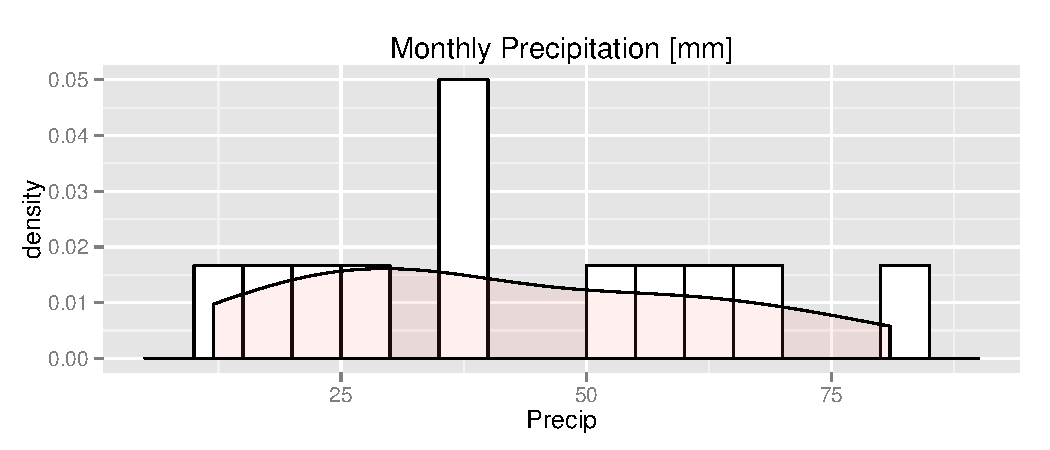
\includegraphics[width=\maxwidth]{figure/1p_den} 

\end{knitrout}
\end{center} \vspace{-0.15in} \caption{Histogram with population density} \end{figure}

      \end{enumerate}
% ===========================================================================
% ===== problem 2 ====
% ===========================================================================
  \item \textbf{Sulphur:}
    \begin{enumerate}
      \item Make stem-and-leaf, histogram, and boxplot for Sulphur data: \\ \\
% ============ figures for (a) =========
\begin{knitrout}
\definecolor{shadecolor}{rgb}{0.969, 0.969, 0.969}\color{fgcolor}\begin{kframe}
\begin{alltt}
\hlkwd{stem}\hlstd{(Sulphur,} \hlkwc{scale} \hlstd{=} \hlnum{4}\hlstd{)}
\end{alltt}
\begin{verbatim}
## 
##   The decimal point is 1 digit(s) to the right of the |
## 
##    1 | 7
##    2 | 5
##    3 | 0448
##    4 | 3
##    5 | 5
##    6 | 34
##    7 | 
##    8 | 
##    9 | 3
##   10 | 
##   11 | 
##   12 | 
##   13 | 5
\end{verbatim}
\end{kframe}
\end{knitrout}

\begin{knitrout}
\definecolor{shadecolor}{rgb}{0.969, 0.969, 0.969}\color{fgcolor}\begin{kframe}
\begin{alltt}
\hlcom{# histogram of Sulphur}
\hlstd{Sulphur.hist} \hlkwb{<-} \hlkwd{ggplot}\hlstd{(d1,} \hlkwd{aes}\hlstd{(}\hlkwc{x} \hlstd{= Sulphur))}
\hlstd{Sulphur.hist} \hlkwb{<-} \hlstd{Sulphur.hist} \hlopt{+} \hlkwd{geom_histogram}\hlstd{(}\hlkwc{binwidth} \hlstd{=} \hlnum{5}\hlstd{)}
\hlstd{Sulphur.hist} \hlkwb{<-} \hlstd{Sulphur.hist} \hlopt{+} \hlkwd{labs}\hlstd{(}\hlkwc{title} \hlstd{=} \hlstr{"Sulphur Concentration [mg/m^2]"}\hlstd{)}
\end{alltt}
\end{kframe}
\end{knitrout}

\begin{figure}[H]  \begin{center}
\begin{knitrout}
\definecolor{shadecolor}{rgb}{0.969, 0.969, 0.969}\color{fgcolor}
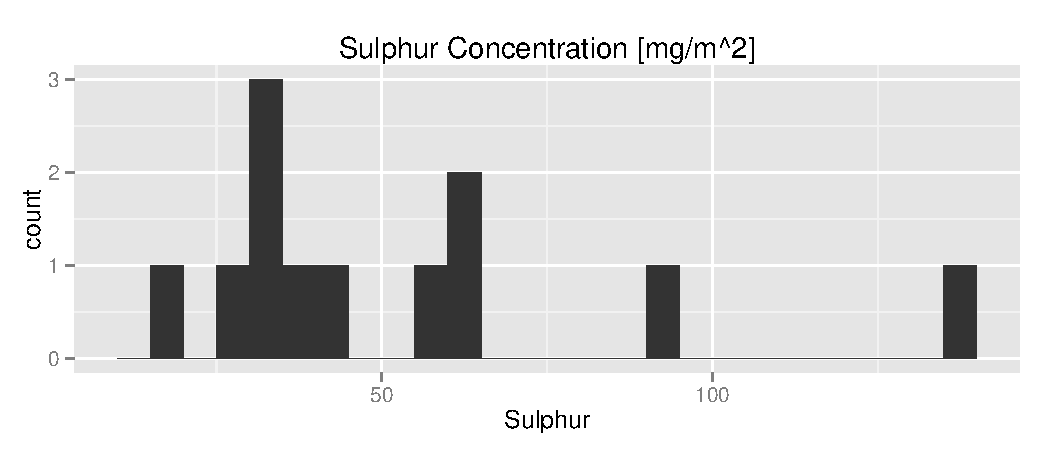
\includegraphics[width=\maxwidth]{figure/2p_hist} 

\end{knitrout}
\end{center} \vspace{-0.25in}\caption{Histogram of Sulphur Data} \end{figure}

\begin{knitrout}
\definecolor{shadecolor}{rgb}{0.969, 0.969, 0.969}\color{fgcolor}\begin{kframe}
\begin{alltt}
\hlstd{Sulphur.box} \hlkwb{<-} \hlkwd{ggplot}\hlstd{(d1,} \hlkwd{aes}\hlstd{(}\hlkwc{x} \hlstd{=} \hlstr{"in"}\hlstd{,} \hlkwc{y} \hlstd{= Sulphur))} \hlcom{# boxplot of Sulphur}
\hlstd{Sulphur.box} \hlkwb{<-} \hlstd{Sulphur.box} \hlopt{+} \hlkwd{geom_boxplot}\hlstd{()}
\hlstd{Sulphur.box} \hlkwb{<-} \hlstd{Sulphur.box} \hlopt{+} \hlkwd{coord_flip}\hlstd{()}
\hlstd{Sulphur.box} \hlkwb{<-} \hlstd{Sulphur.box} \hlopt{+} \hlkwd{labs}\hlstd{(}\hlkwc{title} \hlstd{=} \hlstr{"Sulphur Concentration [mg/m^2]"}\hlstd{)}
\end{alltt}
\end{kframe}
\end{knitrout}

\begin{figure}[H]  \begin{center}
\begin{knitrout}
\definecolor{shadecolor}{rgb}{0.969, 0.969, 0.969}\color{fgcolor}
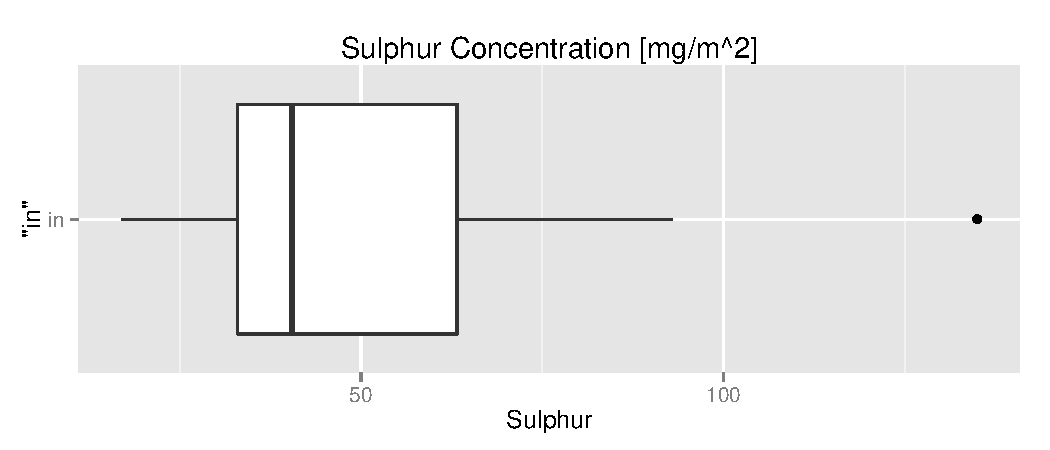
\includegraphics[width=\maxwidth]{figure/2p_box} 

\end{knitrout}
\end{center} \vspace{-0.15in} \caption{Boxplot of Sulphur Data} \end{figure}
% ======== end (a)

      \item Compute mean, median, standard deviation, and IQR for Sulphur data:
        \begin{itemize}
          \item mean: 52.58
          \item median:  40.5
          \item standard deviation:  33.31
          \item inter quartile range:  30.25
        \end{itemize}
\begin{knitrout}
\definecolor{shadecolor}{rgb}{0.969, 0.969, 0.969}\color{fgcolor}\begin{kframe}
\begin{alltt}
\hlkwd{mean}\hlstd{(Sulphur)}    \hlcom{# mean of Sulphur}
\end{alltt}
\begin{verbatim}
## [1] 52.58
\end{verbatim}
\begin{alltt}
\hlkwd{median}\hlstd{(Sulphur)}  \hlcom{# median of Sulphur}
\end{alltt}
\begin{verbatim}
## [1] 40.5
\end{verbatim}
\begin{alltt}
\hlkwd{sd}\hlstd{(Sulphur)}      \hlcom{# standard deviation of Sulphur}
\end{alltt}
\begin{verbatim}
## [1] 33.31
\end{verbatim}
\begin{alltt}
\hlkwd{IQR}\hlstd{(Sulphur)}     \hlcom{# inter quartile range (range for middle half of data)}
\end{alltt}
\begin{verbatim}
## [1] 30.25
\end{verbatim}
\end{kframe}
\end{knitrout}

      \item The mean again is noticeably larger than the median.  An outlier
      exists in the upper end of the data; therefore, I expect the mean to again
      be larger than the median, as the mean is sensitive to skewed data.

      \item The sulphur concentration data are bimodal and skewed right (to the upper end)
        with one outlier.  Based on a "Visual" test, these data are not normally
        distributed (although difficult to asses with limited data).
        These inferences are made apparent with a population frequency curve overlaid
        on a histogram of the population density, as shown in Figure 6.



\begin{figure}[H] \begin{center}
\begin{knitrout}
\definecolor{shadecolor}{rgb}{0.969, 0.969, 0.969}\color{fgcolor}
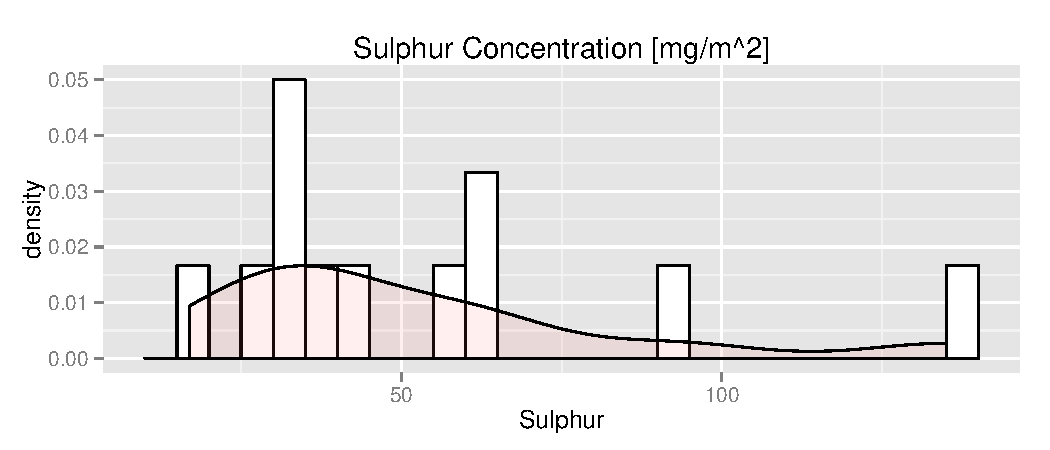
\includegraphics[width=\maxwidth]{figure/2p_den} 

\end{knitrout}
\end{center} \vspace{-0.15in} \caption{Histogram with population density} \end{figure}

      \end{enumerate}

% ===========================================================================
% ===== problem 3 ====
% ===========================================================================
  \item \textbf{Mammals:}

\begin{knitrout}
\definecolor{shadecolor}{rgb}{0.969, 0.969, 0.969}\color{fgcolor}\begin{kframe}
\begin{alltt}
\hlstd{mass.df} \hlkwb{<-} \hlkwd{read.csv}\hlstd{(}\hlstr{"http://statacumen.com/teach/ADA1/ADA1_HW_01_F14-2.csv"}\hlstd{)}
\hlstd{mass} \hlkwb{<-} \hlkwd{as.numeric}\hlstd{(mass.df}\hlopt{$}\hlstd{mass)}
\end{alltt}
\end{kframe}
\end{knitrout}

    \begin{enumerate}
      \item Make stem-and-leaf, histogram, and boxplot for mass data: \\ \\
% ============ figures for (a) =========
\begin{knitrout}
\definecolor{shadecolor}{rgb}{0.969, 0.969, 0.969}\color{fgcolor}\begin{kframe}
\begin{alltt}
\hlkwd{stem}\hlstd{(mass)}
\end{alltt}
\begin{verbatim}
## 
##   The decimal point is 5 digit(s) to the right of the |
## 
##   0 | 00000000000000000000000001111124
##   0 | 9
##   1 | 1
##   1 | 7
##   2 | 
##   2 | 
##   3 | 
##   3 | 
##   4 | 
##   4 | 8
\end{verbatim}
\end{kframe}
\end{knitrout}

\begin{knitrout}
\definecolor{shadecolor}{rgb}{0.969, 0.969, 0.969}\color{fgcolor}\begin{kframe}
\begin{alltt}
\hlcom{# histogram of mass}
\hlstd{mass.hist} \hlkwb{<-} \hlkwd{ggplot}\hlstd{(mass.df,} \hlkwd{aes}\hlstd{(}\hlkwc{x} \hlstd{= mass))}
\hlstd{mass.hist} \hlkwb{<-} \hlstd{mass.hist} \hlopt{+} \hlkwd{geom_histogram}\hlstd{(}\hlkwc{binwidth} \hlstd{=} \hlnum{10000}\hlstd{)}
\hlstd{mass.hist} \hlkwb{<-} \hlstd{mass.hist} \hlopt{+} \hlkwd{labs}\hlstd{(}\hlkwc{title} \hlstd{=} \hlstr{"mass [gram]"}\hlstd{)}
\end{alltt}
\end{kframe}
\end{knitrout}

\begin{figure}[H]  \begin{center}
\begin{knitrout}
\definecolor{shadecolor}{rgb}{0.969, 0.969, 0.969}\color{fgcolor}
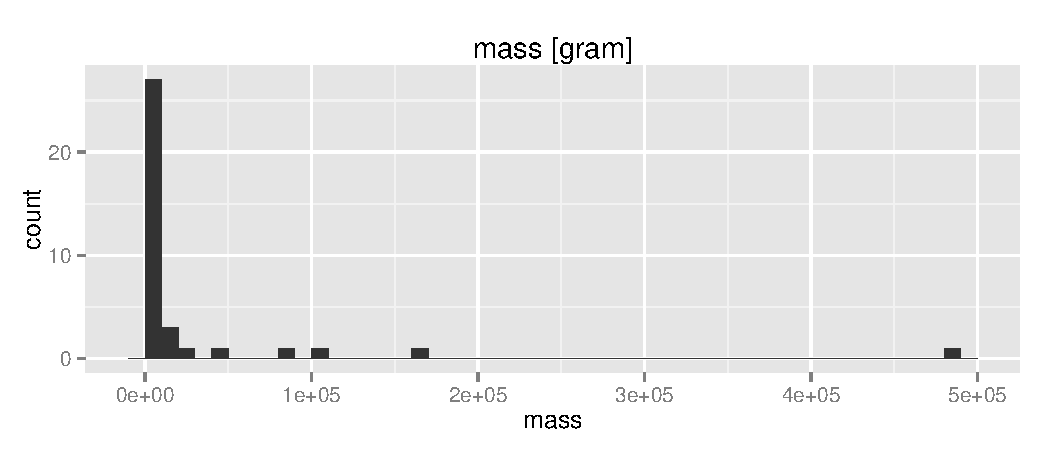
\includegraphics[width=\maxwidth]{figure/3p_hist} 

\end{knitrout}
\end{center} \vspace{-0.25in}\caption{Histogram of mass Data} \end{figure}

\begin{knitrout}
\definecolor{shadecolor}{rgb}{0.969, 0.969, 0.969}\color{fgcolor}\begin{kframe}
\begin{alltt}
\hlstd{mass.box} \hlkwb{<-} \hlkwd{ggplot}\hlstd{(mass.df,} \hlkwd{aes}\hlstd{(}\hlkwc{x} \hlstd{=} \hlstr{"Mammals"}\hlstd{,} \hlkwc{y} \hlstd{= mass))} \hlcom{# boxplot of mass}
\hlstd{mass.box} \hlkwb{<-} \hlstd{mass.box} \hlopt{+} \hlkwd{geom_boxplot}\hlstd{()}
\hlstd{mass.box} \hlkwb{<-} \hlstd{mass.box} \hlopt{+} \hlkwd{coord_flip}\hlstd{()}
\hlstd{mass.box} \hlkwb{<-} \hlstd{mass.box} \hlopt{+} \hlkwd{labs}\hlstd{(}\hlkwc{title} \hlstd{=} \hlstr{"mass [gram]"}\hlstd{)}
\end{alltt}
\end{kframe}
\end{knitrout}

\begin{figure}[H]  \begin{center}
\begin{knitrout}
\definecolor{shadecolor}{rgb}{0.969, 0.969, 0.969}\color{fgcolor}
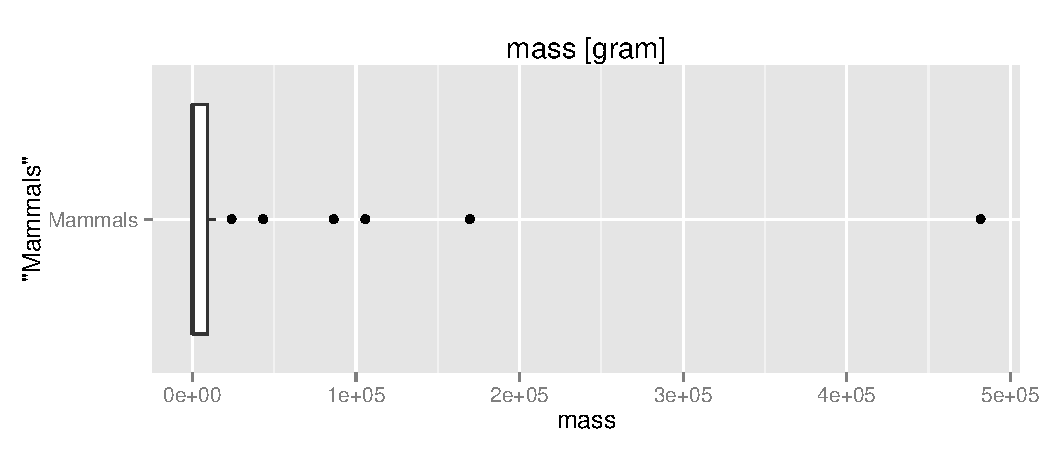
\includegraphics[width=\maxwidth]{figure/3p_box} 

\end{knitrout}
\end{center} \vspace{-0.15in} \caption{Boxplot of mass Data} \end{figure}
% ======== end (a)

      \item Compute mean, median, standard deviation, and IQR for mass data:
        \begin{itemize}
          \item mean: 27,081
          \item median:  92.85
          \item standard deviation:  85,564
          \item inter quartile range:  9,317
        \end{itemize}
\begin{knitrout}
\definecolor{shadecolor}{rgb}{0.969, 0.969, 0.969}\color{fgcolor}\begin{kframe}
\begin{alltt}
\hlkwd{mean}\hlstd{(mass)}    \hlcom{# mean of mass}
\end{alltt}
\begin{verbatim}
## [1] 27081
\end{verbatim}
\begin{alltt}
\hlkwd{median}\hlstd{(mass)}  \hlcom{# median of mass}
\end{alltt}
\begin{verbatim}
## [1] 92.85
\end{verbatim}
\begin{alltt}
\hlkwd{sd}\hlstd{(mass)}      \hlcom{# standard deviation of mass}
\end{alltt}
\begin{verbatim}
## [1] 85564
\end{verbatim}
\begin{alltt}
\hlkwd{IQR}\hlstd{(mass)}     \hlcom{# inter quartile range (range for middle half of data)}
\end{alltt}
\begin{verbatim}
## [1] 9317
\end{verbatim}
\end{kframe}
\end{knitrout}

      \item The mean again is noticeably way larger than the median.  Multiple outliers
      exist in the upper end of the data; therefore, I expect the mean to again
      be larger than the median, as the mean is sensitive to skewed data.

      \item The mass data are multimodal and skewed right (to the upper end)
        with numerous outliers.  Based on a "Visual" test, these data are not normally
        distributed.  Also, the population density is much too low in the IQR to
        be considered normally distributed.
        These inferences are made apparent with a population frequency curve overlaid
        on a histogram of the population density, as shown in Figure 9.



\begin{figure}[H] \begin{center}
\begin{knitrout}
\definecolor{shadecolor}{rgb}{0.969, 0.969, 0.969}\color{fgcolor}
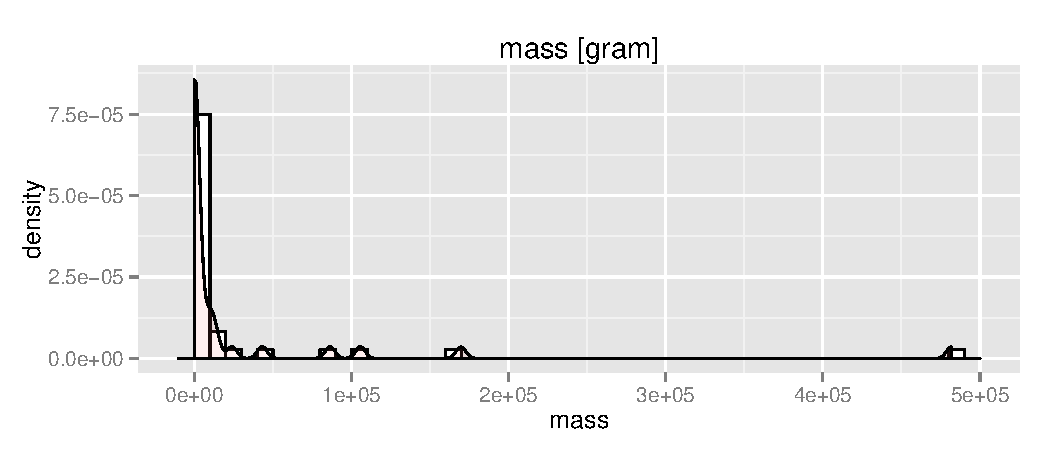
\includegraphics[width=\maxwidth]{figure/3p_den} 

\end{knitrout}
\end{center} \vspace{-0.15in} \caption{Histogram with population density} \end{figure}

      \end{enumerate}

% ===========================================================================
% ===== problem 4 ====
% ===========================================================================
  \item \textbf{log(Mammals):}

\begin{knitrout}
\definecolor{shadecolor}{rgb}{0.969, 0.969, 0.969}\color{fgcolor}\begin{kframe}
\begin{alltt}
\hlstd{logmass.df} \hlkwb{<-} \hlkwd{data.frame}\hlstd{(}\hlkwd{log}\hlstd{(mass.df}\hlopt{$}\hlstd{mass))}
\hlkwd{colnames}\hlstd{(logmass.df)} \hlkwb{<-} \hlstr{"logmass"}
\hlstd{logmass} \hlkwb{<-} \hlkwd{log}\hlstd{(mass)}
\end{alltt}
\end{kframe}
\end{knitrout}

    \begin{enumerate}
      \item Make stem-and-leaf, histogram, and boxplot for log(mass) data: \\ \\
% ============ figures for (a) =========
\begin{knitrout}
\definecolor{shadecolor}{rgb}{0.969, 0.969, 0.969}\color{fgcolor}\begin{kframe}
\begin{alltt}
\hlkwd{stem}\hlstd{(logmass)}
\end{alltt}
\begin{verbatim}
## 
##   The decimal point is at the |
## 
##    0 | 34477
##    2 | 161123335888
##    4 | 473
##    6 | 7139
##    8 | 001246
##   10 | 1746
##   12 | 01
\end{verbatim}
\end{kframe}
\end{knitrout}

\begin{knitrout}
\definecolor{shadecolor}{rgb}{0.969, 0.969, 0.969}\color{fgcolor}\begin{kframe}
\begin{alltt}
\hlcom{# histogram of logmass}
\hlstd{logmass.hist} \hlkwb{<-} \hlkwd{ggplot}\hlstd{(logmass.df,} \hlkwd{aes}\hlstd{(}\hlkwc{x} \hlstd{= logmass))}
\hlstd{logmass.hist} \hlkwb{<-} \hlstd{logmass.hist} \hlopt{+} \hlkwd{geom_histogram}\hlstd{(}\hlkwc{binwidth} \hlstd{=} \hlnum{1}\hlstd{)}
\hlstd{logmass.hist} \hlkwb{<-} \hlstd{logmass.hist} \hlopt{+} \hlkwd{labs}\hlstd{(}\hlkwc{title} \hlstd{=} \hlstr{"logmass [gram]"}\hlstd{)}
\end{alltt}
\end{kframe}
\end{knitrout}

\begin{figure}[H]  \begin{center}
\begin{knitrout}
\definecolor{shadecolor}{rgb}{0.969, 0.969, 0.969}\color{fgcolor}
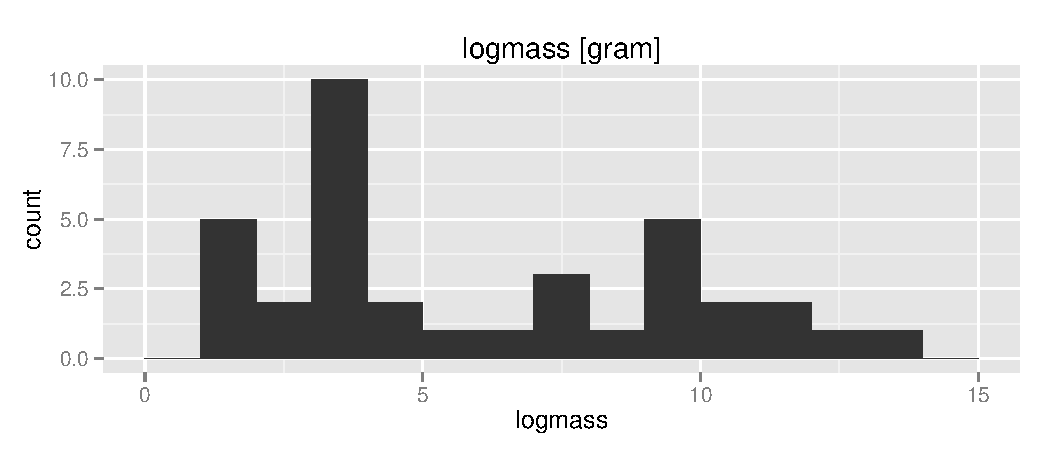
\includegraphics[width=\maxwidth]{figure/4p_hist} 

\end{knitrout}
\end{center} \vspace{-0.25in}\caption{Histogram of log(mass) Data} \end{figure}

\begin{knitrout}
\definecolor{shadecolor}{rgb}{0.969, 0.969, 0.969}\color{fgcolor}\begin{kframe}
\begin{alltt}
\hlstd{logmass.box} \hlkwb{<-} \hlkwd{ggplot}\hlstd{(logmass.df,} \hlkwd{aes}\hlstd{(}\hlkwc{x} \hlstd{=} \hlstr{"Mammals"}\hlstd{,} \hlkwc{y} \hlstd{= logmass))} \hlcom{# boxplot of logmass}
\hlstd{logmass.box} \hlkwb{<-} \hlstd{logmass.box} \hlopt{+} \hlkwd{geom_boxplot}\hlstd{()}
\hlstd{logmass.box} \hlkwb{<-} \hlstd{logmass.box} \hlopt{+} \hlkwd{coord_flip}\hlstd{()}
\hlstd{logmass.box} \hlkwb{<-} \hlstd{logmass.box} \hlopt{+} \hlkwd{labs}\hlstd{(}\hlkwc{title} \hlstd{=} \hlstr{"logmass [gram]"}\hlstd{)}
\end{alltt}
\end{kframe}
\end{knitrout}

\begin{figure}[H]  \begin{center}
\begin{knitrout}
\definecolor{shadecolor}{rgb}{0.969, 0.969, 0.969}\color{fgcolor}
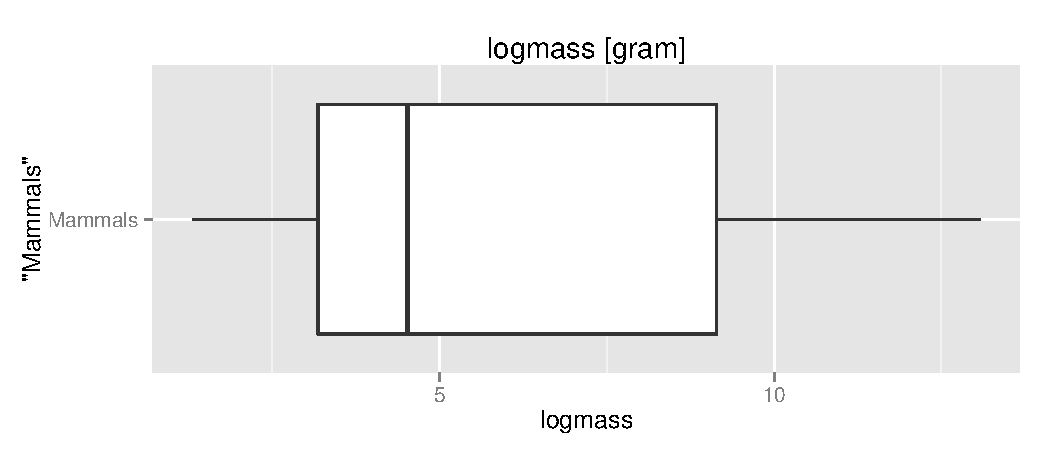
\includegraphics[width=\maxwidth]{figure/4p_box} 

\end{knitrout}
\end{center} \vspace{-0.15in} \caption{Boxplot of logmass Data} \end{figure}
% ======== end (a)

      \item Compute mean, median, standard deviation, and IQR for log(mass) data:
        \begin{itemize}
          \item mean: 5.918
          \item median:  4.522
          \item standard deviation:  3.583
          \item inter quartile range:  5.958
        \end{itemize}
\begin{knitrout}
\definecolor{shadecolor}{rgb}{0.969, 0.969, 0.969}\color{fgcolor}\begin{kframe}
\begin{alltt}
\hlkwd{mean}\hlstd{(logmass)}    \hlcom{# mean of logmass}
\end{alltt}
\begin{verbatim}
## [1] 5.918
\end{verbatim}
\begin{alltt}
\hlkwd{median}\hlstd{(logmass)}  \hlcom{# median of logmass}
\end{alltt}
\begin{verbatim}
## [1] 4.522
\end{verbatim}
\begin{alltt}
\hlkwd{sd}\hlstd{(logmass)}      \hlcom{# standard deviation of logmass}
\end{alltt}
\begin{verbatim}
## [1] 3.583
\end{verbatim}
\begin{alltt}
\hlkwd{IQR}\hlstd{(logmass)}     \hlcom{# inter quartile range (range for middle half of data)}
\end{alltt}
\begin{verbatim}
## [1] 5.958
\end{verbatim}
\end{kframe}
\end{knitrout}

      \item The mean again is noticeably larger than the median.  No
      exist in the data; therefore.  I expect the mean to again
      be larger than the median, as the mean is sensitive to skewed data and these
      data are skewed to the right.

      \item The log(mass) data are bimodal and skewed right (to the upper end)
        with no outliers (a value would need to be extremely large to be considered
        an outlier in log space e.g., $e^{20}$).
        Based on a "Visual" test, these data are not normally
        distributed, as they are bimodal.
        These inferences are made apparent with a population frequency curve overlaid
        on a histogram of the population density, as shown in Figure 12.



\begin{figure}[H] \begin{center}
\begin{knitrout}
\definecolor{shadecolor}{rgb}{0.969, 0.969, 0.969}\color{fgcolor}
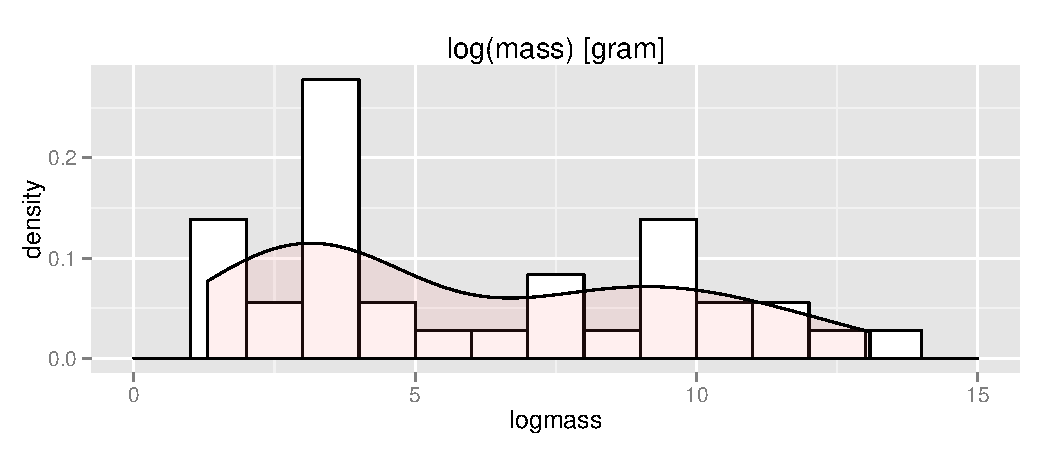
\includegraphics[width=\maxwidth]{figure/4p_den} 

\end{knitrout}
\end{center} \vspace{-0.15in} \caption{Histogram with population density} \end{figure}

      \end{enumerate}
    \end{enumerate}
\end{document}
